Consider the one-dimensional, transient (i.e. time-dependent) 
heat conduction equation without heat generating sources

\[
\rho C_p \frac{\partial T}{\partial t} 
= \frac{\partial }{\partial x} \left(  k  \frac{\partial T}{\partial x} \right)
\]
where $\rho$ is density, $C_p$ heat capacity, $k$ thermal conductivity, $T$ temperature, 
$x$ distance, and $t$ time. 

If the thermal conductivity, density and heat capacity are constant over the model domain, 
the equation can be simplified to a diffusion equation:
\[
\frac{\partial T}{\partial t} =  \kappa \frac{\partial^2 T}{\partial x^2} 
\]
where $\kappa=k/\rho c_p$ is the heat diffusivity.

We wish to solve this PDE in time and space (provided the appropriate 
boundary conditions have been given). 


\begin{center}
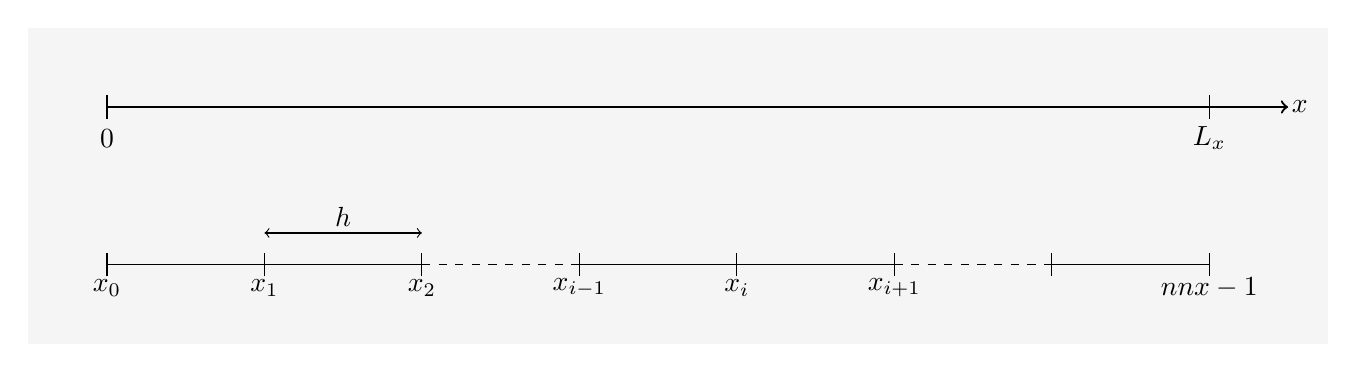
\begin{tikzpicture}
\draw[fill=gray!8,gray!8](0,0) rectangle (16.5,4);
%\draw[step=0.5cm,gray,very thin] (0,0) grid (16.5,4); %background grid
\node[] at (16.15,3) {$x$};
\node[] at (1,2.6) {$0$};
\node[] at (15,2.6) {$L_x$};
\draw[-] (1,2.85) -- (1,3.15) ; 
\draw[-] (15,2.85) -- (15,3.15) ; 
\draw[thick,->] (1,3) -- (16,3) ; 

%\draw[fill=gray!13,gray!13](1,1) rectangle (8,3);
%\draw[thick] (1,1) -- (5,1) -- (5,4) -- (1,4) -- cycle;  

\draw[-] (1,1) -- (5,1) ; 
\draw[dashed] (5,1) -- (7,1) ; 
\draw[-] (7,1) -- (11,1) ; 
\draw[dashed] (11,1) -- (13,1) ; 
\draw[-] (13,1) -- (15,1) ; 

\draw[-] (1,0.85) -- (1,1.15) ; 
\draw[-] (3,0.85) -- (3,1.15) ; 
\draw[-] (5,0.85) -- (5,1.15) ; 
\draw[-] (7,0.85) -- (7,1.15) ; 
\draw[-] (9,0.85) -- (9,1.15) ; 
\draw[-] (11,0.85) -- (11,1.15) ; 
\draw[-] (13,0.85) -- (13,1.15) ; 
\draw[-] (15,0.85) -- (15,1.15) ; 

\node[] at (7,0.7) {$x_{i-1}$};
\node[] at (9,0.7) {$x_i$};
\node[] at (11,0.7) {$x_{i+1}$};

\node[] at (1,0.7) {$x_0$};
\node[] at (3,0.7) {$x_1$};
\node[] at (5,0.7) {$x_2$};
\node[] at (15,0.7) {$nnx-1$};

\draw[<->] (3,1.4) -- (5,1.4) ; 
\node[] at (4,1.6) {$h$};

\end{tikzpicture}


\end{center}

The derivative of temperature with regards to time can be approximated
with a forward finite difference approximation as
\[
\frac{\partial T}{\partial t} 
\simeq \frac{T_{i}^{n+1}-T_i^n}{t^{n+1}-t^n} 
= \frac{T_{i}^{n+1}-T_i^n}{\delta t} 
\]
where $\delta t$ is the time step, i.e. the time between two consecutive 
measurements (the equivalent of $h$ in space).

$n$ represents the temperature at the current time step whereas $n+1$
represents the new (future) temperature. The subscript $i$ refers to the location in space.

Both $n$ and $i$ are integers; $n$ varies from 1 to nstep (total number of time steps)
and $i$ varies from 0 to $nnx-1$ (where $nnx$ is the total number of grid points in $x$-direction).

The spatial derivative is replaced by a central FD approximation
\[
\frac{\partial^2 T}{\partial x^2} 
\simeq \frac{T_{i+1}^n - 2T_i^n + T_{i-1}^n}{h^2}
\]
We obtain
\[
\frac{T_{i}^{n+1}-T_i^n}{\delta t} 
= \kappa \frac{T_{i+1}^n - 2T_i^n + T_{i-1}^n}{h^2}
\]
and finally
\[
\boxed{
T_i^{n+1}=T_i^n + \delta t \; \kappa \frac{T_{i+1}^n - 2T_i^n + T_{i-1}^n}{h^2}
}
\]

Because the temperature at the current time step $n$ is known,
we can compute the new temperature without solving any additional equations.
Such a scheme is an {\bf explicit} finite difference method and
was made possible by the choice to evaluate the temporal derivative with forward differences.

\begin{center}


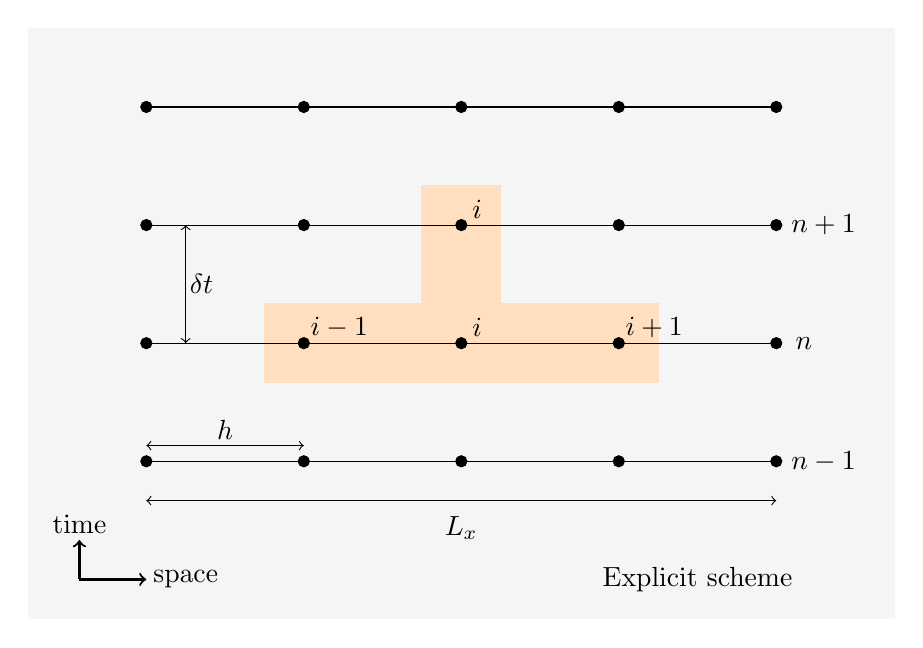
\begin{tikzpicture}
\draw[fill=gray!8,gray!8](-0.5,0) rectangle (10.5,7.5);


\draw[fill=orange,orange!25](2.5,3) rectangle (7.5,4);
\draw[fill=orange,orange!25](4.5,4) rectangle (5.5,5.5);
%\draw[step=0.5cm,gray,very thin] (0,0) grid (10.5,7.5); %background grid

\draw[black,fill=black] (1,2)  circle (2pt);
\draw[black,fill=black] (3,2)  circle (2pt);
\draw[black,fill=black] (5,2)  circle (2pt);
\draw[black,fill=black] (7,2)  circle (2pt);
\draw[black,fill=black] (9,2)  circle (2pt);

\draw[black,fill=black] (1,3.5)  circle (2pt);
\draw[black,fill=black] (3,3.5)  circle (2pt);
\draw[black,fill=black] (5,3.5)  circle (2pt);
\draw[black,fill=black] (7,3.5)  circle (2pt);
\draw[black,fill=black] (9,3.5)  circle (2pt);

\draw[black,fill=black] (1,5)  circle (2pt);
\draw[black,fill=black] (3,5)  circle (2pt);
\draw[black,fill=black] (5,5)  circle (2pt);
\draw[black,fill=black] (7,5)  circle (2pt);
\draw[black,fill=black] (9,5)  circle (2pt);

\draw[black,fill=black] (1,6.5)  circle (2pt);
\draw[black,fill=black] (3,6.5)  circle (2pt);
\draw[black,fill=black] (5,6.5)  circle (2pt);
\draw[black,fill=black] (7,6.5)  circle (2pt);
\draw[black,fill=black] (9,6.5)  circle (2pt);

\draw[-] (1,2) -- (9,2) ;
\draw[-] (1,3.5) -- (9,3.5) ;
\draw[-] (1,5) -- (9,5) ;
\draw[-] (1,6.5) -- (9,6.5) ;

\draw[<->] (1,2.2) -- (3,2.2) ;
\node[] at (2,2.4) {$h$};

\draw[<->] (1.5,3.5) -- (1.5,5) ;
\node[] at (1.7,4.25) {$\delta t$};

\draw[<->] (1,1.5) -- (9,1.5) ;
\node[] at (5,1.15) {$L_x$};

\draw[thick,->] (0.15,0.5) -- (1,0.5) ;
\draw[thick,->] (0.15,0.5) -- (0.15,1) ;
\node[] at (1.5,0.5) {space};
\node[] at (0.15,1.2) {time};

\node[] at (3.45,3.7) {$i-1$};
\node[] at (5.2,3.7) {$i$};
\node[] at (7.45,3.7) {$i+1$};
\node[] at (5.2,5.2) {$i$};

\node[] at (9.6,2) {$n-1$};
\node[] at (9.35,3.5) {$n$};
\node[] at (9.6,5) {$n+1$};

\node[] at (8,0.5) {Explicit scheme};
\end{tikzpicture}
                                      


\end{center}


In order to solve the original PDE equation we need to
\begin{itemize}
\item prescribe an initial temperature field
\item prescribe two boundary conditions 
\end{itemize}
Such requirements hold also in the discrete world. 

We know that this numerical scheme will converge to the exact solution for
small $h$ and $\delta t$ because it has been shown to be {\color{olive}consistent} - 
that its discretization process
can be reversed, through a Taylor series expansion, to recover the governing partial differential equation -
and because it is {\color{olive}stable} for certain values of
$h$ and $\delta t$: any spontaneous perturbations in the solution (such as round-off error) 
will either be bounded or will decay.

Concretely, we will prescribe an initial temperature field $T_i^0$ for $i=0,nnx-1$.
For example:

\begin{center}


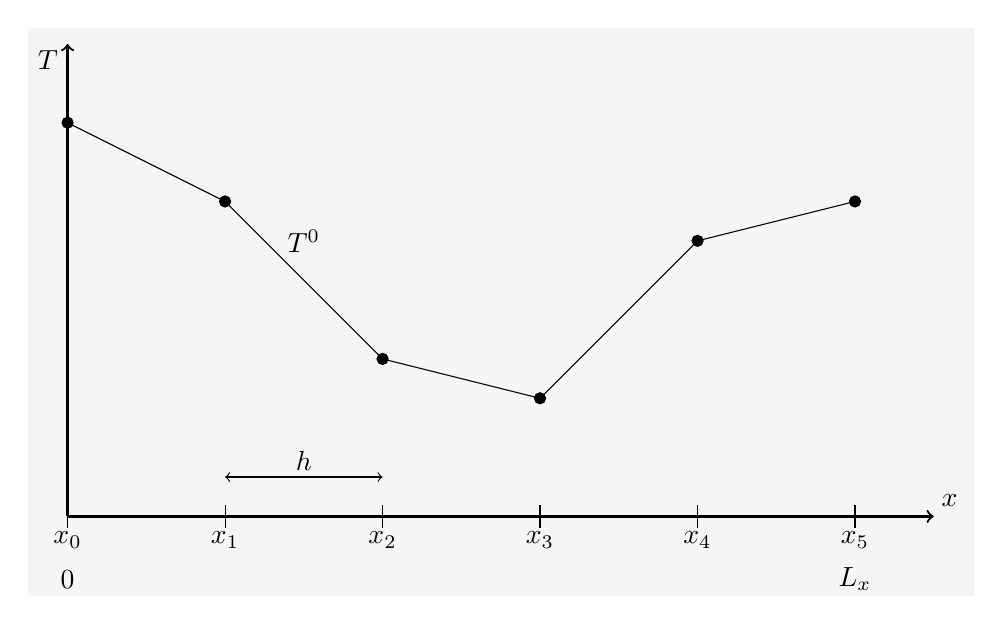
\begin{tikzpicture}
\draw[fill=gray!8,gray!8](0.5,0) rectangle (12.5,7.2);
%\draw[step=0.5cm,gray,very thin] (0,0) grid (13,7); %background grid

\draw[thick,->] (1,1) -- (12,1) ; 
\draw[thick,->] (1,1) -- (1,7) ; 


\node[] at (12.2,1.2) {$x$};
\node[] at (1,0.2) {$0$};
\node[] at (11,0.2) {$L_x$};
\node[] at (0.75,6.8) {$T$};

\draw[black,fill=black] (1,6)  circle (2pt);
\draw[black,fill=black] (3,5)  circle (2pt);
\draw[black,fill=black] (5,3)  circle (2pt);
\draw[black,fill=black] (7,2.5)  circle (2pt);
\draw[black,fill=black] (9,4.5)  circle (2pt);
\draw[black,fill=black] (11,5)  circle (2pt);

\draw[-] (1,6) -- (3,5) -- (5,3) -- (7,2.5) -- (9,4.5) -- (11,5); 
\node[] at (4,4.5) {$T^0$};

\draw[-] (1,0.85) -- (1,1.15) ; 
\draw[-] (3,0.85) -- (3,1.15) ; 
\draw[-] (5,0.85) -- (5,1.15) ; 
\draw[-] (7,0.85) -- (7,1.15) ; 
\draw[-] (9,0.85) -- (9,1.15) ; 
\draw[-] (11,0.85) -- (11,1.15) ; 
\node[] at (1,0.7) {$x_0$};
\node[] at (3,0.7) {$x_1$};
\node[] at (5,0.7) {$x_2$};
\node[] at (7,0.7) {$x_3$};
\node[] at (9,0.7) {$x_4$};
\node[] at (11,0.7) {$x_5$};
\draw[<->] (3,1.5) -- (5,1.5) ;  
\node[] at (4,1.7) {$h$};
\end{tikzpicture}


\end{center}

Then, we will be able to compute the new temperature of (for example) 
node 3 at time $t=1\cdot \delta t$ 
(i.e. $T_3^1$) with 
\[
T_3^{1}=T_3^0 + \delta t \; \kappa \frac{T_{4}^0 - 2T_3^0 + T_{2}^0}{h^2}
\]
Note that $T_0$ and $T_5$ cannot be computed by means of the above equation, 
which is not a problem because both these values are actually the chosen 
boundary conditions. 


The main drawback of the explicit approach is that stable solutions are
obtained {\it only} when
\[
0 < \frac{2\kappa \delta t}{h^2} \leq1
\]
or,
\[
\delta t \leq \frac{h^2}{2 \kappa}
\]
If this condition is not satisfied, the solution becomes {\color{olive} unstable}, starts to
wildly oscillate and ultimately 'blows up'. We will observe this during the practicals. 

The stability condition means that the maximum time step needs to be smaller than the time it
takes for an anomaly to diffuse across the grid (nodal) spacing $h$.
The explicit solution is an example of a {\color{olive} conditionally stable method}
that only leads to well behaved solutions if a criterion like the one above is satisfied.

\begin{center}
\begin{minipage}[t]{0.77\textwidth}
\par\noindent\rule{\textwidth}{0.4pt}

\begin{center}

\includegraphics[width=0.8cm]{images/garftr} \\
{\color{orange}Exercise 2}
\end{center}

We are going to solve the 1D diffusion equation with the explicit method
for the following physical setup: The domain is $L_x=1$km long, 
it is maintained at a temperature $T=100\degree$C at $x=0$ and at a temperature
$T=200\degree$C at $x=L_x$. The initial temperature is $T(x,t=0)=123$
and $\kappa=10^{-6}$. 
Time stepping will be carried out until steady state is reached.

\par\noindent\rule{\textwidth}{0.4pt}
\end{minipage}
\end{center}

An alternative approach is an {\bf implicit} finite difference scheme, where the spatial derivatives
of the Laplacian are evaluated (at least partially) at the new time step.

We then use the backward difference for the time derivative:
\[
\frac{\partial T}{\partial t} 
= \frac{T_{i}^{n}-T_i^{n-1}}{\delta t} 
\]
so that
\[
\frac{T_{i}^{n}-T_i^{n-1}}{\delta t} 
= \kappa \frac{T_{i+1}^n - 2T_i^n + T_{i-1}^n}{h^2}
\]
Note that this is often rewritten as follows in order to keep the unknwowns at time $n+1$:
\[
\frac{T_{i}^{n+1}-T_i^{n}}{\delta t} 
= \kappa \frac{T_{i+1}^{n+1} - 2T_i^{n+1} + T_{i-1}^{n+1}}{h^2}
\]

It is a fully implicit scheme where the time derivative is taken backward.
Let us define the dimensionless parameter $s$ as follows:
\[
s=\frac{\kappa \delta t}{h^2}
\]
The previous equation can be rearranged as follows:
\[
\boxed{
-s T_{i+1}^{n+1} + (1+2s) T_{i}^{n+1} - s T_{i-1}^{n+1} = T_i^{n}
}
\]

\begin{center}
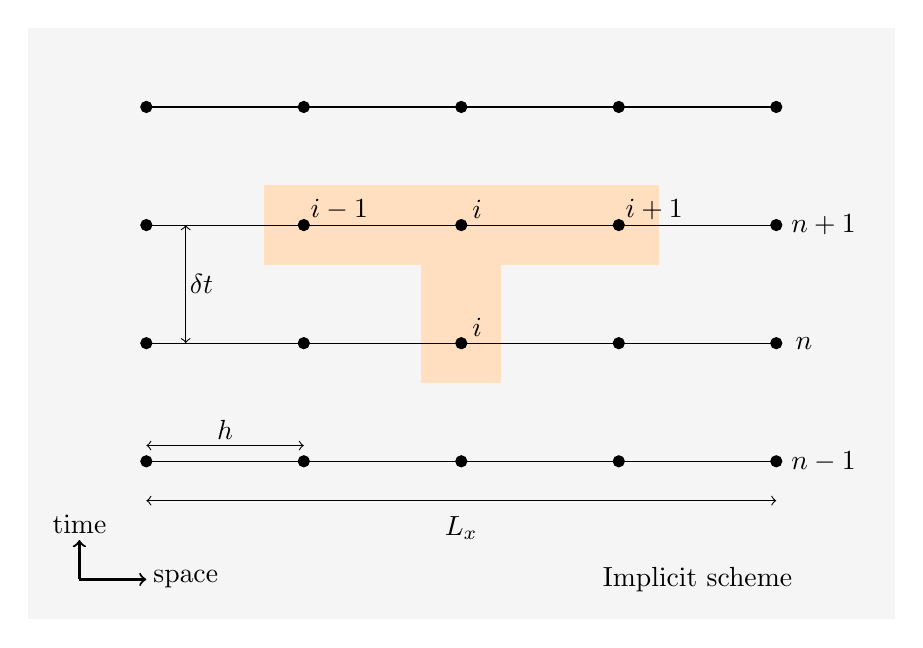
\begin{tikzpicture}
\draw[fill=gray!8,gray!8](-0.5,0) rectangle (10.5,7.5);

\draw[fill=orange,orange!25](2.5,4.5) rectangle (7.5,5.5);
\draw[fill=orange,orange!25](4.5,3) rectangle (5.5,4.5);
%\draw[step=0.5cm,gray,very thin] (0,0) grid (10.5,7.5); %background grid

\draw[black,fill=black] (1,2)  circle (2pt);
\draw[black,fill=black] (3,2)  circle (2pt);
\draw[black,fill=black] (5,2)  circle (2pt);
\draw[black,fill=black] (7,2)  circle (2pt);
\draw[black,fill=black] (9,2)  circle (2pt);

\draw[black,fill=black] (1,3.5)  circle (2pt);
\draw[black,fill=black] (3,3.5)  circle (2pt);
\draw[black,fill=black] (5,3.5)  circle (2pt);
\draw[black,fill=black] (7,3.5)  circle (2pt);
\draw[black,fill=black] (9,3.5)  circle (2pt);

\draw[black,fill=black] (1,5)  circle (2pt);
\draw[black,fill=black] (3,5)  circle (2pt);
\draw[black,fill=black] (5,5)  circle (2pt);
\draw[black,fill=black] (7,5)  circle (2pt);
\draw[black,fill=black] (9,5)  circle (2pt);

\draw[black,fill=black] (1,6.5)  circle (2pt);
\draw[black,fill=black] (3,6.5)  circle (2pt);
\draw[black,fill=black] (5,6.5)  circle (2pt);
\draw[black,fill=black] (7,6.5)  circle (2pt);
\draw[black,fill=black] (9,6.5)  circle (2pt);

\draw[-] (1,2) -- (9,2) ;
\draw[-] (1,3.5) -- (9,3.5) ;
\draw[-] (1,5) -- (9,5) ;
\draw[-] (1,6.5) -- (9,6.5) ;

\draw[<->] (1,2.2) -- (3,2.2) ;
\node[] at (2,2.4) {$h$};

\draw[<->] (1.5,3.5) -- (1.5,5) ;
\node[] at (1.7,4.25) {$\delta t$};

\draw[<->] (1,1.5) -- (9,1.5) ;
\node[] at (5,1.15) {$L_x$};

\draw[thick,->] (0.15,0.5) -- (1,0.5) ;
\draw[thick,->] (0.15,0.5) -- (0.15,1) ;
\node[] at (1.5,0.5) {space};
\node[] at (0.15,1.2) {time};

\node[] at (3.45,5.2) {$i-1$};
\node[] at (5.2,3.7) {$i$};
\node[] at (7.45,5.2) {$i+1$};
\node[] at (5.2,5.2) {$i$};

\node[] at (9.6,2) {$n-1$};
\node[] at (9.35,3.5) {$n$};
\node[] at (9.6,5) {$n+1$};

\node[] at (8,0.5) {Implicit scheme};
\end{tikzpicture}
                                                                                                                                                                                                                 



\end{center}



Note that in this case we no longer have an explicit relationship for 
$T^{n+1}_{i-1}$, $T^{n+1}_i$ and $T^{n+1}_{i+1}$.
Instead, we have to solve a {\color{olive}linear system of equations}, which is discussed further below.

The main advantage of implicit methods is that there are no restrictions on the time step,
the fully implicit scheme is {\bf unconditionally stable}.
This does not mean that it is accurate. 
Taking large time steps may result in an inaccurate solution for features with
small spatial scales!

For any application, it is therefore always a good idea to check the 
results by decreasing the time step
until the solution does not change anymore (this is called a {\color{olive}convergence check}), and 
to ensure the
method can deal with small and large scale features robustly at the same time.

Once again let us look at things with a very concrete approach. Let us discretise the 
domain of length $L_x$ with 6 cells, i.e. $i=0,\dots 6$ ($nnx=7$).
We also prescribe the following boundary conditions (remember it is a 2nd order derivative in space, 
so we need two of them): $T(x=0)=T_0=0$ and $T(x=L_x)=T_6=100$ (we assume that they 
do not change with time for simplicity). Finally we assume that we 
know $T_i^0$ for all $i$ and we wish to compute $T_i^1$.

We then have:
\begin{eqnarray}
T_0^1 &=& 0 \nn\\
-s T_{2}^{1} + (1+2s) T_{1}^{1} - s T_{0}^{1} &=& T_1^{0} \nn\\
-s T_{3}^{1} + (1+2s) T_{2}^{1} - s T_{1}^{1} &=& T_2^{0} \nn\\
-s T_{4}^{1} + (1+2s) T_{3}^{1} - s T_{2}^{1} &=& T_3^{0} \nn\\
-s T_{5}^{1} + (1+2s) T_{4}^{1} - s T_{3}^{1} &=& T_4^{0} \nn\\
-s T_{6}^{1} + (1+2s) T_{5}^{1} - s T_{4}^{1} &=& T_5^{0} \nn\\
T_6^1 &=& 100\nn
\end{eqnarray}
or, 
\[
\underbrace{
\left(
\begin{array}{ccccccc}
1 & 0 & 0 & 0 & 0 & 0 & 0  \\
-s & 1+2s & -s & 0 & 0 & 0 & 0 \\
0 & -s & 1+2s & -s & 0 & 0 & 0 \\
0 & 0 & -s & 1+2s & -s & 0 & 0 \\
0 & 0 & 0 & -s & 1+2s & -s & 0 \\
0 & 0 & 0 & 0 & -s & 1+2s & -s \\
0 & 0 & 0 & 0 & 0 & 0 & 1
\end{array}
\right)
}_{\bm A}
\cdot
\underbrace{
\left(
\begin{array}{ccccccc}
T_0^1 \\ T_1^1 \\ T_2^1 \\ T_3^1 \\ T_4^1 \\ T_5^1 \\ T_6^1  
\end{array}
\right)
}_{\vec{T}}
=
\underbrace{
\left(
\begin{array}{ccccccc}
0 \\ T_1^0\\ T_2^0\\ T_3^0\\ T_4^0\\ T_5^0 \\ 100
\end{array}
\right)
}_{\vec{b}}
\]

As opposed to the explicit approach we must solve a linear system which size is given 
by the total number of nodes/points $nnx$ in order to compute a new temperature field.

In summary, an implicit method requires us to solve ${\bm A}\cdot\vec{T} = \vec{b}$ with
\begin{itemize}
\item ${\bm A}$ is a $nnx \times nnx$  {\color{olive}sparse} matrix,
\item ${\vec b}$ is a known vector of size $nnx$ (often called the 'right-hand side', or {\color{olive} rhs})
\item ${\vec T}$ the vector of unknowns.
\end{itemize}



Looking at
\[
-s T_{i+1}^{n+1} + (1+2s) T_{i}^{n+1} - s T_{i-1}^{n+1} = T_i^{n}
\]
and dividing by $-s$ and letting $\delta t \rightarrow \infty$, we obtain:
\[
T_{i+1}^{n+1} -2 T_{i}^{n+1} + T_{i-1}^{n+1} = 0
\]
which is a central difference approximation of the steady state solution
\[
\frac{\partial^2 T }{\partial x^2}=0
\]
Therefore, the fully implicit scheme will always yield the right equilibrium solution 
but may not capture small scale, transient features.


\begin{center}
\begin{minipage}[t]{0.77\textwidth}
\par\noindent\rule{\textwidth}{0.4pt}

\begin{center}

\includegraphics[width=0.8cm]{images/garftr} \\
{\color{orange}Exercise 3}
\end{center}

This is exactly the same exercise as Exercise 2 but we 
are going to solve the 1D diffusion equation with the implicit method
this time. 

\par\noindent\rule{\textwidth}{0.4pt}
\end{minipage}
\end{center}


\paragraph{Crank-Nicolson scheme} 
It turns out that this fully implicit method is second order accurate in space but 
only first order accurate in time,
i.e. the error goes as ${\cal O}(h^3,\delta t^2)$.   VERIFY !!!!

It is possible to write down a scheme which is second order accurate both in time and in space
(i.e. ${\cal O}(h^3, \delta t^3))$, e.g. the {\color{olive}Crank-Nicolson} scheme 
which is unconditionally stable (The method was developed by John Crank and Phyllis Nicolson 
in the mid 20th century\footnote{\url{https://en.wikipedia.org/wiki/Crank-Nicolson_method}}).

The Crank-Nicolson method is the time analog of central spatial differences and is given by

\[
\frac{T_{i}^{n+1}-T_i^n}{\delta t} 
= \frac{\kappa}{2} \left[
\frac{T_{i+1}^{n} - 2T_i^{n} + T_{i-1}^{n}}{h^2}
+
\frac{T_{i+1}^{n+1} - 2T_i^{n+1} + T_{i-1}^{n+1}}{h^2}
\right]
\]
We define $s=\kappa \delta t/ 2h^2$ so that the equation above can be rearranged as follows :
\[
\boxed{
-s T_{i+1}^{n+1} + (1+2s) T_{i}^{n+1} - s T_{i-1}^{n+1} = 
s T_{i+1}^{n} + (1-2s) T_{i}^{n} + s T_{i-1}^{n} 
}
\]


Any partially implicit method is more tricky to compute as we need to infer the future solution 
at time $n+1$ by solution (inversion) of a system of linear equations based on the known solution at time $n$. 

\begin{center}

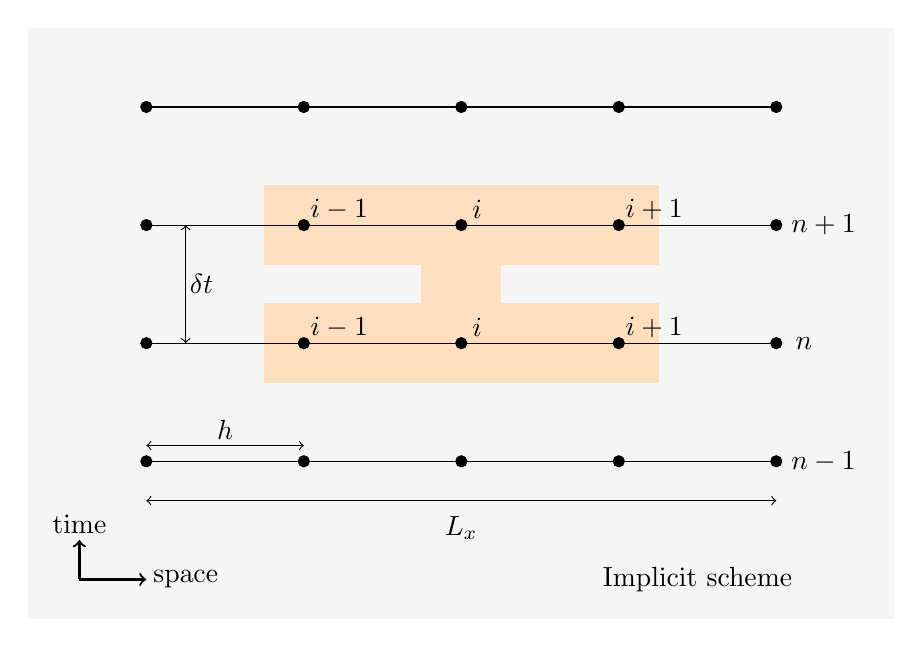
\begin{tikzpicture}
\draw[fill=gray!8,gray!8](-0.5,0) rectangle (10.5,7.5);


\draw[fill=orange,orange!25](2.5,4.5) rectangle (7.5,5.5);
\draw[fill=orange,orange!25](4.5,3) rectangle (5.5,4.5);
\draw[fill=orange,orange!25](2.5,3) rectangle (7.5,4);

%\draw[step=0.5cm,gray,very thin] (0,0) grid (10.5,7.5); %background grid

\draw[black,fill=black] (1,2)  circle (2pt);
\draw[black,fill=black] (3,2)  circle (2pt);
\draw[black,fill=black] (5,2)  circle (2pt);
\draw[black,fill=black] (7,2)  circle (2pt);
\draw[black,fill=black] (9,2)  circle (2pt);

\draw[black,fill=black] (1,3.5)  circle (2pt);
\draw[black,fill=black] (3,3.5)  circle (2pt);
\draw[black,fill=black] (5,3.5)  circle (2pt);
\draw[black,fill=black] (7,3.5)  circle (2pt);
\draw[black,fill=black] (9,3.5)  circle (2pt);

\draw[black,fill=black] (1,5)  circle (2pt);
\draw[black,fill=black] (3,5)  circle (2pt);
\draw[black,fill=black] (5,5)  circle (2pt);
\draw[black,fill=black] (7,5)  circle (2pt);
\draw[black,fill=black] (9,5)  circle (2pt);

\draw[black,fill=black] (1,6.5)  circle (2pt);
\draw[black,fill=black] (3,6.5)  circle (2pt);
\draw[black,fill=black] (5,6.5)  circle (2pt);
\draw[black,fill=black] (7,6.5)  circle (2pt);
\draw[black,fill=black] (9,6.5)  circle (2pt);

\draw[-] (1,2) -- (9,2) ;
\draw[-] (1,3.5) -- (9,3.5) ;
\draw[-] (1,5) -- (9,5) ;
\draw[-] (1,6.5) -- (9,6.5) ;

\draw[<->] (1,2.2) -- (3,2.2) ;
\node[] at (2,2.4) {$h$};

\draw[<->] (1.5,3.5) -- (1.5,5) ;
\node[] at (1.7,4.25) {$\delta t$};

\draw[<->] (1,1.5) -- (9,1.5) ;
\node[] at (5,1.15) {$L_x$};

\draw[thick,->] (0.15,0.5) -- (1,0.5) ;
\draw[thick,->] (0.15,0.5) -- (0.15,1) ;
\node[] at (1.5,0.5) {space};
\node[] at (0.15,1.2) {time};

\node[] at (3.45,3.7) {$i-1$};
\node[] at (3.45,5.2) {$i-1$};
\node[] at (5.2,3.7) {$i$};
\node[] at (7.45,5.2) {$i+1$};
\node[] at (7.45,3.7) {$i+1$};
\node[] at (5.2,5.2) {$i$};

\node[] at (9.6,2) {$n-1$};
\node[] at (9.35,3.5) {$n$};
\node[] at (9.6,5) {$n+1$};

\node[] at (8,0.5) {Implicit scheme};
\end{tikzpicture}
                                                                                                                                                                                                                 




\end{center}


\begin{center}
\begin{minipage}[t]{0.77\textwidth}
\par\noindent\rule{\textwidth}{0.4pt}

\begin{center}

\includegraphics[width=0.8cm]{images/garftr} \\
{\color{orange}Exercise 4}
\end{center}

\par\noindent\rule{\textwidth}{0.4pt}
\end{minipage}
\end{center}





